\PassOptionsToPackage{numbers}{natbib} % passing an option to  natbib before tufte-book
\documentclass[justified,openany,nofonts]{tufte-book}

\usepackage{teacherEd}

\usepackage{framed}
\usepackage{comment}

%\newenvironment{teachingnote}{\begin{framed}\begin{itshape}\begin{bfseries}\noindent Teaching Note:}{\end{bfseries}\end{itshape}\end{framed}}
%\newcommand{\teachingnotes}{With Teaching Notes}
\excludecomment{teachingnote}
\newcommand{\teachingnotes}{}

%\def\fixnote#1{\begin{framed}{\color{red}Fixnote: #1}\end{framed}}  % Allows insertion of red notes about needed edits
\def\fixnote#1{}

%%% This sets how the enumerate command works
\renewcommand{\theenumi}{$(\mathrm{\arabic{enumi}})$}
\renewcommand{\labelenumi}{\theenumi}

\title{Parallels \\ in Geometry \\ (Supplements)}
\author{\teachingnotes}
\publisher{Math 1166:  Spring 2015 \\ This document was typeset on \today.}
%\date{}



\begin{document}
\def\document#1{} %% Needed to add standards
\maketitle

\setcounter{tocdepth}{1}
\tableofcontents

\setcounter{secnumdepth}{2} % turn on numbering for parts and chapters

%% Put main text here


\newpage

\chapter{Toward Congruence and Similarity}
Need to renumber so the section number is correct. 

\section{Similar Triangles}

One day when aloof old Professor Rufus was trying to explain similar
triangles to his class, he merely wrote
\[
\tri ABC \sim \tri A'B'C' \qquad\Leftrightarrow \qquad\begin{array}{l}
\angle A \simeq \angle A'\\
\angle B \simeq \angle B' \\
\angle C \simeq \angle C'
\end{array}
\]
and walked out of the room.

\begin{question} 
Can you give $3$ much needed examples of similar triangles? 
\end{question}
\QM

\begin{question} 
Devise a way to use folding and tracing constructions to help explore this notion
of similar triangles.
\end{question}
\QM

Another day when aloof old Professor Rufus was trying to explain
similar triangles to his class, he merely wrote
\[
\tri ABC \sim \tri A'B'C' \qquad\Leftrightarrow \qquad
\begin{array}{l}
AB = k\cdot A'B'\\
BC = k\cdot B'C' \\
CA = k\cdot C'A'
\end{array}
\]
and walked out of the room.

\begin{question} 
Can you give $3$ much needed examples of similar triangles? 
\end{question}
\QM

\begin{question} 
Devise a way to use folding and tracing constructions to help explore this notion
of similar triangles.
\end{question}
\QM



\begin{question} 
What's going on in aloof old Professor Rufus' head?  (I realize that
this is a dangerous question!)  Why are his explanations so different?
\end{question}
\QM


%%%%%%%%%%%%%%%%%%%%%%%%%%%%%%%%%%%%%%%%%%%
%% UPSHOT: Either defintion is good for this course. There
%% will/should-be handouts proving AA and SSS for similarity, hence
%% proving they are the same.
%%%%%%%%%%%%%%%%%%%%%%%%%%%%%%%%%%%%%%%%%%%



\subsection{Theorems for Similar Triangles}

In this section we will show that that \textbf{both} definitions of similar
triangles given above are \textbf{equivalent}.  We'll start with a gentle
question:

\begin{question} What is the formula for the area of a triangle?
\end{question}
\QM

Using merely the formula for the area of a triangle, we (meaning you)
will explain why the following important theorem is true. Throughout this 
discussion we will use the convention that when we
write $AB$ we mean the \textit{length} of the segment $AB$.


\begin{theorem}[Parallel-Side] 
\index{Parallel-Side Theorem}\index{Theorem!Parallel-Side}
Given:
\[
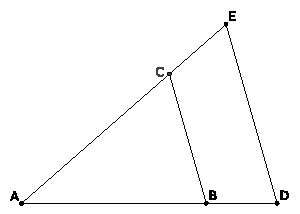
\includegraphics{../graphics/split1.pdf}
\]
If side $BC$ is parallel to side $DE$, then
\[
\frac{AB}{AD} = \frac{AC}{AE}.
\] 
\end{theorem}

\begin{question}
Can you tell me in English what this theorem says? Provide some
examples of this theorem in action.
\end{question}
\QM

Now we (meaning you) are going to explore a bit. See if answering
these questions sheds light on this.

\begin{question} 
If $h$ is the height of $\tri ABC$, find a formula for the areas of
$\tri ABC$ and $\tri ADC$.
\[
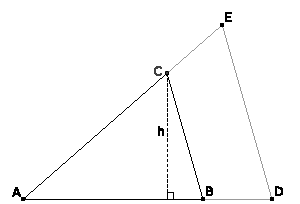
\includegraphics{../graphics/split2.pdf} \qquad 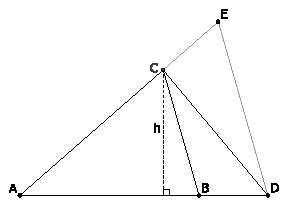
\includegraphics{../graphics/split3.pdf}
\]
\end{question}
\QM

\begin{question} 
If $g$ is the height of $\tri ACB$, find a formula for the areas of
$\tri ACB$ and $\tri AEB$.
\[
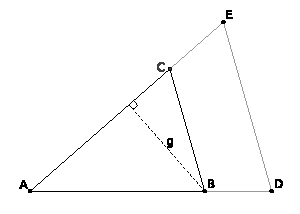
\includegraphics{../graphics/split4.pdf} \qquad 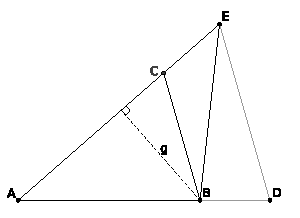
\includegraphics{../graphics/split5.pdf}
\]
\end{question}
\QM


\begin{question} Explain why 
\[
\mathrm{Area}(\tri ABC) = \mathrm{Area}(\tri ACB).
\]
\end{question}
\QM

\begin{question} Explain why 
\[
\mathrm{Area}(\tri CBE) = \mathrm{Area}(\tri CBD).
\]
Big hint: Use the fact that you have two parallel sides! Draw a
picture to help clarify your explanation.
\end{question}
\QM

\begin{question} Explain why 
\[
\mathrm{Area}(\tri ADC)= \mathrm{Area}(\tri AEB).
\]
\end{question}
\QM

\begin{question}
Explain why
\[
\frac{\mathrm{Area}(\tri ABC)}{\mathrm{Area}(\tri ADC)} = \frac{ \mathrm{Area}(\tri ACB)}{\mathrm{Area}(\tri AEB)}
\]
\end{question}
\QM

\begin{question} Compute and simplify both of the following expressions:
\[
\frac{\mathrm{Area}(\tri ABC)}{\mathrm{Area}(\tri ADC)} \qquad\text{and}\qquad\frac{ \mathrm{Area}(\tri ACB)}{\mathrm{Area}(\tri AEB)}
\]
\end{question}
\QM


\begin{question} How can you conclude that: 
\[
\frac{AB}{AD} = \frac{AC}{AE}
\]
\end{question}
\QM

\begin{question} 
Why is it important that line $DE$ is parallel to line $CB$?
\end{question}
\QM


\begin{question} 
Can you sketch out (in words) how the questions above prove the Parallel-Side
Theorem?
\end{question}
\QM

Now comes the moment of truth. 
\begin{question}
Can you use the Parallel-Side Theorem to explain why if you know that
if you have two triangles, $\tri ABC$ and $\tri A'B'C'$ with:
\begin{align*}
\angle A &\simeq \angle A'\\
\angle B &\simeq \angle B' \\
\angle C &\simeq \angle C'
\end{align*}
then we must have that
\begin{align*}
AB &= k\cdot A'B'\\
BC &= k\cdot B'C'\\
CA &= k\cdot C'A'
\end{align*}
\end{question}
\QM






\subsubsection{The Converse}

The converse of the Parallel-Side Theorem states:

\begin{theorem}[Split-Side]\index{Split-Side Theorem}\index{Theorem!Split-Side} 
Given:
\[
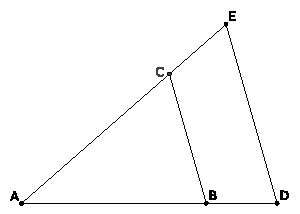
\includegraphics{../graphics/split1.pdf}
\]
If side $BC$ intersects (splits) the sides of $\tri ADE$ so that
\[
\frac{AB}{AD} = \frac{AC}{AE},
\] 
then side $BC$ is parallel to side $DE$.
\end{theorem}

\begin{question} 
How could you investigate this theorem using any of the construction
techniques above?
\end{question}
\QM

Now we (meaning you) will answer questions in the hope that they will
help us see why the above theorem is true.

\begin{question}
Suppose that you \textbf{doubt} that side $BC$ is parallel to side $DE$. Explain
how to place a point $C'$ on side $AE$ so that side $BC'$ is
parallel to line $DE$. Be sure to sketch the situation(s).
\end{question}
\QM

\begin{question} 
You now have a triangle $\tri ADE$ whose sides are split by a line
$BC'$ such that the line $BC'$ is parallel to line $DE$. What does the
Parallel-Side Theorem have to say about this?
\end{question}
\QM

\begin{question} What can you conclude about points $C$ and $C'$?
\end{question}
\QM


\begin{question} 
What does this tell you about the Split-Side Theorem?
\end{question}
\QM




Let's see if you can put this all together:
\begin{question}
Can you use the Split-Side Theorem to explain why if you know that
if you have two triangles, $\tri ABC$ and $\tri A'B'C'$ with:
\begin{align*}
AB &= k\cdot A'B'\\
BC &= k\cdot B'C'\\
CA &= k\cdot C'A'
\end{align*}
then we must have that
\begin{align*}
\angle A &\simeq \angle A'\\
\angle B &\simeq \angle B' \\
\angle C &\simeq \angle C'
\end{align*}
\end{question}
\QM

Putting all of our work above together, we may now say the following:





\begin{definition}\index{similar triangles} 
Two triangles $\tri ABC$ and $\tri A'B'C'$ are said to be
\textbf{similar} if either equilvalent condition holds:
\[
\begin{array}{l}
\angle A \simeq \angle A'\\
\angle B \simeq \angle B' \\
\angle C \simeq \angle C'
\end{array}
\qquad\text{or}\qquad
\begin{array}{l}
AB = k\cdot A'B'\\
BC = k\cdot B'C' \\
CA = k\cdot C'A'
\end{array}
\]
\end{definition}



\subsubsection{SAS-Similarity Theorem}







\begin{theorem}[SAS-Similarity Theorem]
\index{Theorem!SAS Similarity}\index{SAS-Similarity Theorem} Knowing
the ratio of the lengths of two sides and the measure of the angle
between them, determines a triangle up to similarity. In pictures, we have something like:
\[
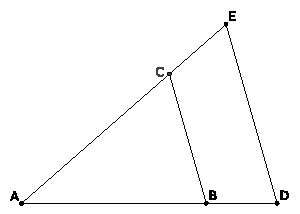
\includegraphics{../graphics/split1.pdf}
\]
\[
\frac{AB}{AC} = \frac{AD}{AE} \qquad\Rightarrow\qquad \tri ABC \simeq \tri ADE.
\]
\end{theorem}

\begin{question} What does this mean, ``up to similarity?''
\end{question}
\QM

Let's see if we (meaning you) can get to the bottom of why this
theorem is true. This time, you're going to produce the
illustrations. Use folding and tracing why not!

\begin{question}
Fold any triangle. Now fold another triangle sharing one of the angles
so that the ratio of the lengths of the sides are the same in both
triangles. The sides touching the angle should share folds. You should
see some parallel lines. Which theorem above says that this should
happen?
\end{question}
\QM

\begin{question} 
What do we know about parallel lines crossing another line?
\end{question}
\QM

\begin{question} 
Can you sketch out (in words) how the questions above prove the SAS-Similarity
Theorem?
\end{question}
\QM


\subsection{A Meaning of Multiplication}

Do you ever sit around asking yourself what different things
\textit{mean}? For example, ``What does being happy really mean?'' In
mathematics we don't dare try to tackle a brain-buster like that
one. Instead we try to focus on simple problems.

\begin{question} What can multiplication mean? 
\end{question}
\QM

I have no idea how you might have answered that question. Anyhow,
maybe you can answer the next questions:

\begin{question} 
Can you give multiplication meaning involving groups of groups or
something of the sort?
\end{question}
\QM

\begin{question} 
Can you give multiplication meaning involving areas or something of
the sort?
\end{question}
\QM

\begin{question}
Compare and contrast the two meanings of multiplication given above.
\end{question}

OK---all of this is fine and good, but we one little problem. If
numbers by themselves ``mean'' lengths and numbers multiplied together
``mean'' areas, how do we do something like this:
\[
\underbrace{3}_\text{length} + \underbrace{4\cdot 5}_\text{area}?
\]


I say we can use similar triangles to save the day!


\begin{question} 
Can you somehow give ``meaning'' to multiplication using similar
triangles? Hint: One of them should have a side of length $1$.
\end{question}
\QM

  % Bart's notes

% Section 4.5. Length, area, and volume under scaling (with problems)
% Section 5.5. Functions and more functions


%
 \chapter{CCSS Grade 8 to HS Geometry}  

\section{Grade 8}
In school mathematics, transformations and symmetry have typically been small niche topics, separate from each other, separate from most of the rest of school mathematics, and receiving little curricular attention.  Congruence, on the other hand, is a more prominent idea that begins informally in the elementary grades as ``same shape, same size'' and culminates in high school with axioms, theorems, and proofs.  

Understand congruence and similarity using physical models, transparencies, or geometry software.
\standard{8.G.1} \standard{8.G.1a} \standard{8.G.1b} \standard{8.G.1c}
\standard{8.G.2}
\standard{8.G.3}
\standard{8.G.4}
\standard{8.G.5}

Understand and apply the Pythagorean Theorem.
\standard{8.G.6}
\standard{8.G.7}
\standard{8.G.8}

Solve real-world and mathematical problems involving volume of
cylinders, cones, and spheres.
\standard{8.G.9}

\section{High School Geometry}
In school mathematics, transformations and symmetry have typically been small niche topics, separate from each other, separate from most of the rest of school mathematics, and receiving little curricular attention.  Congruence, on the other hand, is a more prominent idea that begins informally in the elementary grades as ``same shape, same size'' and culminates in high school with axioms, theorems, and proofs.  

Experiment with transformations in the plane
\standardhs{G-CO.1}
\standardhs{G-CO.2}
\standardhs{G-CO.3}
\standardhs{G-CO.4}
\standardhs{G-CO.5}

Understand congruence in terms of rigid motions
\standardhs{G-CO.6}
\standardhs{G-CO.7}
\standardhs{G-CO.8}

Prove geometric theorems
\standardhs{G-CO.9}
\standardhs{G-CO.10}
\standardhs{G-CO.11}

Make geometric constructions
\standardhs{G-CO.12}
\standardhs{G-CO.13}

Understand similarity in terms of similarity transformations
\standardhs{G-SRT.1}\standardhs{G-SRT.1a}\standardhs{G-SRT.1b}
\standardhs{G-SRT.2}
\standardhs{G-SRT.3}

Prove theorems involving similarity
\standardhs{G-SRT.4}
\standardhs{G-SRT.5}

Define trigonometric ratios and solve problems involving right
triangles
\standardhs{G-SRT.6}
\standardhs{G-SRT.7}
\standardhs{G-SRT.8}

Apply trigonometry to general triangles
\standardhs{G-SRT.9}
\standardhs{G-SRT.10}
\standardhs{G-SRT.11}


\appendix

\renewcommand{\theenumi}{$(\mathrm{\alph{enumi}})$}
\renewcommand{\labelenumi}{\theenumi}
\chapter{Supplemental Activities}

%\setcounter{page}{1}
%\setcounter{section}{43}


% Activities in draft form or to be developed

% tessellation activity for early in the term
% Walking and turning a la Beckmann
% some version of the CMP dilation activity
% scaling volume
% connecting the dots for parametric?  
% 
\newpage 

\section{Circular Trigonometry}
As we have seen, right triangle trigonometry is restricted to acute angles.  But angles are often obtuse, so it is quite useful to extend trigonometry to angles greater than $90^\circ$.  Here is one approach:  Place the angle with the vertex at the origin in the coordinate and with one side of the angle (the initial side) along the positive $x$-axis.  Measure to the other side of the angle (the terminal side) as a counter-clockwise rotation about the origin.   

%\begin{prob}
%Now we can find the area of a triangle given two sides and an angle.\standardhs{G-SRT.9}  
%\end{prob}
%
%% Laws of Sines and Cosines \standardhs{G-SRT.10}, \standardhs{G-SRT.11}

Because angles are often about rotation, angles greater than $180^\circ$ can make sense, too.  And negative angles can describe rotation in the opposite direction.  If we consider the angle to change continuously, then rotation about the origin creates a situation that repeats every $360^\circ$.  This repetition provides the foundation for modeling lots of repetitive (periodic) contexts in the real world.  For this modeling, we need \emph{circular trigonometry}, which turns out to be much cleaner if (1) angles are measured not in degrees but in a more ``natural'' unit, called radians; and (2) we use \emph{the unit circle}, which is a circle of radius 1 centered at the origin.   The steps are as follows:  

\begin{enumerate}
\item Understanding radian measure.\standardhs{G-C.5}, \standardhs{F-TF.1}

\item Using the unit circle to extend trigonometry to angles of any measure.\standardhs{F-TF.2}

\item Choosing and using trig functions to model periodic phenomena.\standardhs{F-TF.5}

\end{enumerate}

\fixnote{Complete this activity or section.}
% Fluency finding trig functions of special angles in radian measure.\standardhs{F-TF.3}



%  Unused activities

%\newpage
\section{Louie Llama and Regular Polygons} 

Louie Llama is a very curious llama.\index{Louie Llama} He knows that
each angle of a regular $3$-gon is $60^\circ$. He also knows that each
angle of a regular $4$-gon is $90^\circ$. But what he really wants to
know, are the measure of each angle of a regular $n$-gon. In this
activity we'll see if we can answer this question.


\begin{prob} 
Draw a picture of Louie Llama rotated $90^\circ$ counterclockwise.
\end{prob}

\begin{prob} 
Draw a picture of Louie Llama rotated $180^\circ$ counterclockwise.
\end{prob}

\begin{prob} 
Draw a picture of Louie Llama rotated $360^\circ$ counterclockwise.
\end{prob}

\begin{prob} Sometimes Louie Llama likes to walk around lines he finds:
\[
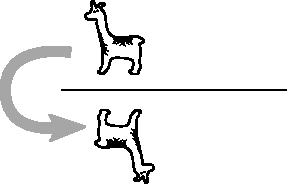
\includegraphics{../graphics/llamaLines.pdf}
\]
Through what angle did Louie Llama just rotate?
\end{prob}

Again, we're going to watch Louie Llama go for a walk. Draw yourself
any a regular $3$-gon. When Louie Llama walks around corners he
rotates. Check it out:
\[
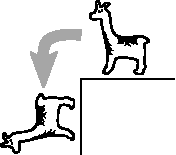
\includegraphics{../graphics/llamaCorner.pdf}
\]
Since your $3$-gon is regular, each of its angles has measure
$\theta$. 
\begin{prob} 
Sketch Louie Llama walking around our $3$-gon. As he goes around a
corner, through what angle does Louie Llama rotate?
\end{prob}

\begin{prob}
Find the measure of each angle of a $3$-gon. Explain your reasoning.
\end{prob}

\begin{prob}
Sketch a regular $4$-gon and find the measure of each angle of a
$4$-gon. Explain your reasoning.
\end{prob}


\begin{prob}
Sketch a regular $5$-gon and find the measure of each angle of a
$5$-gon. Explain your reasoning.
\end{prob}


\begin{prob}
Sketch a regular $6$-gon and find the measure of each angle of a
$6$-gon. Explain your reasoning.
\end{prob}


Now it is time to generalize!

\begin{prob}
Sketch a regular $n$-gon and find the measure of each angle of a
$n$-gon. Explain your reasoning. Note, your answer should be a formula.
\end{prob}



\newpage
\section{Apothem} %% remove * if added to main notes

Draw yourself a picture of a happy little equilateral triangle. Do
it---seriously.  Some people might call an equilateral triangle a
\textit{regular 3-gon}.

\begin{prob} 
What is an \textit{$n$-gon}? Give some relevant and revealing examples
and nonexamples.
\end{prob}

\begin{prob} 
When discussing $n$-gons, what are the allowable values for $n$?
\end{prob}

\begin{prob} 
What is a \textit{regular $n$-gon}? Give some relevant and revealing
examples and nonexamples.
\end{prob}


\begin{dfn} 
A segment connecting the intersection of any two perpendicular
bisectors of sides of a polygon to either of those sides is called an
\textbf{apothem}\index{apothem}.
\end{dfn}

\begin{prob}
Can you tell me in English what this defintion says? Provide some
examples of this definition in action.
\end{prob}



\begin{prob} 
Now consider some regular $n$-gon. Use \textsl{GeoGebra} to construct
apothems.
\end{prob}



\begin{prob}
Given a polygon, if you know the side length and the length of the
apothems, how do you find the area of your polygon? 
\end{prob}


\begin{prob}
Fix a value for $n$. Then use \textsl{GeoGebra} to help you fill in
the following table for various lengths of apothems.
\begin{center}
\begin{tabular}{|c||c|c|c|c|}\hline
$n$-gon & Apothem & Side & Perimeter & Area  \\\hline\hline
 \rule[0mm]{0mm}{7mm}\hspace{15mm}  &  & &  &  \\ \hline
 \rule[0mm]{0mm}{7mm}\hspace{15mm} &  & &  &  \\ \hline
 \rule[0mm]{0mm}{7mm}\hspace{15mm} &  & &  &  \\ \hline
 \rule[0mm]{0mm}{7mm}\hspace{15mm} &  & &  &  \\ \hline
 \rule[0mm]{0mm}{7mm}\hspace{15mm} &  & &  &  \\ \hline
 \rule[0mm]{0mm}{7mm}\hspace{15mm} &  & &  &  \\ \hline
 \rule[0mm]{0mm}{7mm}\hspace{15mm} &  & &  &  \\ \hline
\end{tabular}
\end{center}
\end{prob}

\begin{prob}
If $a$ is the length of the apothem, $P$ is the perimeter, and $A$ is
the area of the regular polygon, can you give a formula relating all
three of these quantities?
%\[
%A = \frac{pa}{2}
%\]
\end{prob}


% \newpage
\section{Subs at Sea}

Take your favorite $n$-gon and consider the group of symmetries, call it $G$. Write out the group table for $G$. Got it? Good.

\begin{prob} Let $\mat{M}$ be an element of your group. Define
\[
C(\mat{M}) = \{\text{all elements of $G$ that commute with $\mat{M}$}\}.
\]
For every element $\mat{M}\in G$, write out $C(\mat{M})$. Make some
observations.
\end{prob}

\begin{prob}
Exactly which elements of $G$ commute with everything?
\end{prob}

\begin{prob}
Repeat the exercises above for a different group.
\end{prob}

\begin{prob}
Are the sets $C(\mat{M})$ groups themselves? Explain why or why not.
\end{prob}

\begin{prob}
For any given $\mat{M}$, what do you notice about the number of
elements found in $C(\mat{M})$?
\end{prob}


   % Subs at Sea.  Center of an element of a group
\newpage
\section{Golden Ratio} %% remove * if added to main notes


\begin{question} Is the golden ratio constructible?\index{golden!ratio} 
\end{question}
\QM

Well 
\[
\phi =\frac{1 + \sqrt{5}}{2},
\]
so of course it is. But, how do you actually construct it? Here is an easy way:

\begin{construction}[Golden Ratio]\index{compass and straightedge!golden ratio}\index{golden!ratio!compass and straightedge} \hfill
\begin{enumerate}
\item Consider a unit on a line.
\item Construct a perpendicular of unit length at the right end point of the unit.
\item Bisect the original unit.
\item Draw an arc, centered at the point found in Step $3$ that goes 
through the top of the perpendicular drawn in Step $2$.
\item The segment starting at the left end of the unit and ending at the point found in Step $4$ is of length $\phi$.
\end{enumerate}
\[

\includegraphics{../graphics/phi.pdf}
\]
\end{construction}


\begin{question}\index{compass and straightedge!pentagon}\index{pentagon}How how do you construct a regular pentagon? 
\end{question}
One way is to use golden triangles:\index{golden!triangle}
\[
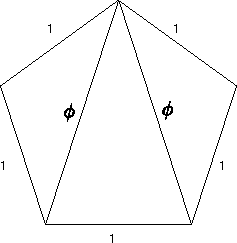
\includegraphics{../graphics/pentagon.pdf}
\]

What about other regular $n$-gons?  \index{Gauss, Carl Friedrich}Carl
Friedrich Gauss, one of the greatest mathematicians of all time,
solved this problem when he was 18. He did this around the year 1800,
nearly 2000 years after the time of the Greeks.  How did he do it?  He
thought of constructions algebraically as we have been doing. Using
these methods, he discovered this theorem:


\begin{theorem}[Gauss]\label{T:gauss}  One can construct a regular $n$-gon if $n\ge 3$ and 
\[
n= 2^i \cdot p_1\cdot p_2\cdots p_j
\]
where each subscripted $p$ is a distinct prime number of the form
\[
2^{(2^k)}+1
\]
where  $i$, $j$, and $k$ are nonnegative integers.
\end{theorem}\index{prime numbers}

Around thirty years later, Wantzel\index{Wantzel, Pierre} proved that
these were the only regular polygons that could be constructed.

\begin{question} Find $i$, $j$, and $k$ for a regular $3$-gon, $4$-gon, $5$-gon, and $6$-gon.
\end{question}
\QM

\newpage
\section{Rule the Day} 
       
In this activity, we try to understand what the ``act of measuring is'' a
quantity. In particular, we will try to draw out common measurement ...

\begin{prob} 
2. What are standard units that people typically use when measuring
length, area, and volume?  Are they related to one another in some
way(s)?  What other kind of units could be used to measure, say, area?
Why might they be less “popular”?
\end{prob}



\begin{prob}
When we measure the ``amount quantity'' of a set of apples, the
``amount'' measurement is done with the unit being the type of object
the set consists of.  Why can't we do that when measuring length,
area, volume, time, weight, or angle?  What do we do instead?
\end{prob}



\chapter{Supplemental Problems}
\newpage

\section{Midterm 1 Review Problems}

\begin{prob}
Describe Euclid's construction for an equilateral triangle, and explain
why it works.
\end{prob}

\begin{prob}
Use the picture below to show that a pair of medians intersects at a point 2/3 of the way from the vertex to the opposite side.  Then use that fact to argue that the three medians must be concurrent.  
$$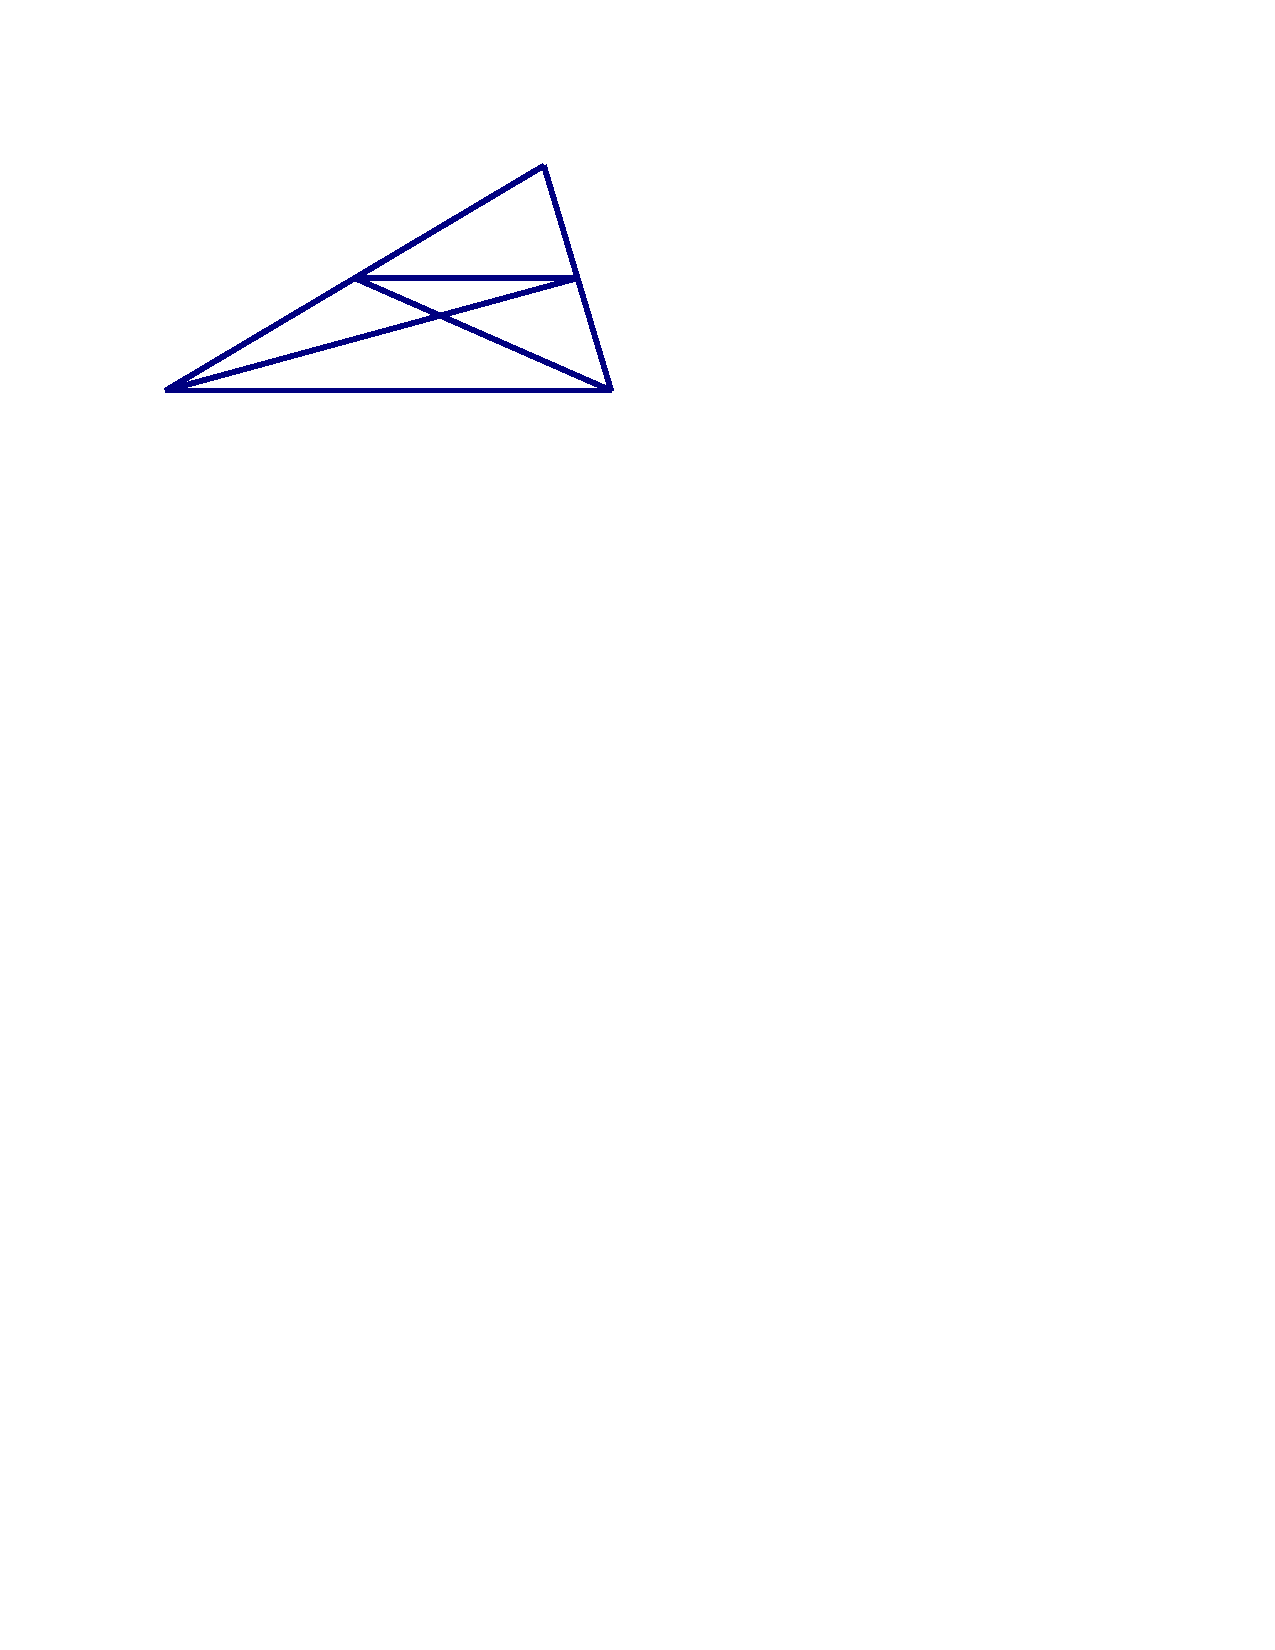
\includegraphics[width=2.5in]{../graphics/median1.pdf}$$
\end{prob}

\begin{prob}
Prove that the points on an angle bisector are \emph{exactly those} that are equidistant from the sides of the angle. 
\end{prob}

\begin{prob}
Show that, given any three non-collinear points in the Euclidean plane, there is a unique circle passing through the three points.
\end{prob}

\begin{prob}
Given a circle, give a construction that finds its center.
\end{prob}

\begin{prob}
State and prove a condition on any quadrilateral that is inscribed in a circle.  
\end{prob}

\begin{prob}
Construct a tangent line from a point outside a given circle to the circle.
\end{prob}

\begin{prob}
Give an informal derivation of the relationship between the circumference and area of a circle. 
\end{prob}

\begin{prob}
Prove:  If a quadrilateral is a parallelogram, then opposite sides are congruent.
\end{prob}

\begin{prob}
Prove:  If opposite sides of a quadrilateral are congruent, then it is a parallelogram.
\end{prob}



\newpage

\section{Midterm 2 Review Problems}

\begin{prob}
During a solar eclipse we see that the apparent diameter of the Sun and Moon are nearly equal. If the Moon is around 240,000 miles from Earth, the Moon's diameter is about 2000 miles, and the Sun's diameter is about 865,000 miles how far is the Sun from the Earth?
\begin{enumerate}
\item Draw a relevant (and helpful) picture showing the important points of this problem.
\item Write an expression that gives the solution to this problem---show all work.
\end{enumerate}
\end{prob}

\begin{prob}
A typical adult male gorilla is about 5.5 feet tall and weighs about 400 pounds. Suppose King Kong was about 22 feet tall and proportioned like a typical adult male gorilla.
\begin{enumerate}
\item Write an expression that approximates King Kong's weight. Briefly explain your reasoning.
\item The circumference of the neck of a typical adult male gorilla is 36 inches. Approximately what would be the circumference of King Kong's neck? Briefly explain your reasoning.
\item Suppose an Ohio State sweatshirt for a typical adult male gorilla requires 3 square yards of fabric.  Approximately how much fabric would be required for an Ohio State sweatshirt for King Kong?  Briefly explain your reasoning.
\end{enumerate}
\end{prob}

\begin{prob}
Brenah is drinking fruit punch from a glass shaped like an inverted cone.  Suppose the glass has a height 5 in. and a base of radius 2 in.  What is the volume of the glass?  What is the height of the fruit punch when the glass is half full?  Generalize your result for any glass shaped like an inverted cone.  
\end{prob}

\begin{prob}
A cup has a circular opening, a circular base, and circular cross sections at every height parallel to the base.  The opening has a diameter of 9 cm, the base has a diameter of 6 cm, and the cup is 12 cm high.  
What is the volume of the cup?  Explain your reasoning.  
If the cup is filled to half its height, what fraction of the cup's volume is filled?  Explain your reasoning.  
\end{prob}

\begin{prob}
Suppose you use a photocopier to enlarge a figure to 125\% of its original size.  What is the scale factor of the enlargement?  What happens to areas under the enlargement?  If you lost the original figure, what reduction percentage would you use on the enlargment to create a figure congruent to the original?  What is the scale factor for the reduction?  
\end{prob}

\begin{prob}
Explain how the following picture ``proves'' the Pythagorean Theorem.
\[
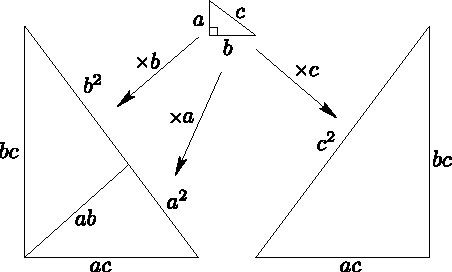
\includegraphics[scale=0.8]{../graphics/pbpdilation.pdf}
\]
\end{prob}

\begin{prob}
Here is a right triangle, note it is \textbf{not} drawn to scale:
\[
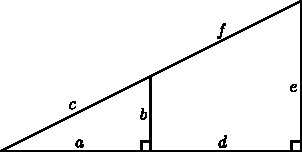
\includegraphics{../graphics/origamiSimQ.pdf}
\]
Solve for all unknowns in the following cases.
\begin{enumerate}
\item $a = 3$, $b = ?$, $c = ?$, $d = 12$, $e = 5$, $f = ?$
\item $a = ?$, $b = 3$, $c = ?$, $d =8$, $e = 13$, $f = ?$
\item $a = 7$, $b = 4$, $c = ?$, $d =?$, $e = 11$, $f = ?$
\item $a = 5$, $b = 2$, $c = ?$, $d =6$, $e = ?$, $f = ?$
\end{enumerate}
In each case explain your reasoning.
\end{prob}

\begin{prob}
Describe a general (and foolproof) way of demonstrating that any two parabolas are similar.
\end{prob}

\begin{prob}
Prove that the angle sum of a triangle is $180^\circ$.
\end{prob}

\begin{prob}
Construct a tangent line from a point outside a given circle to the circle.
\end{prob}

\begin{prob}
Explain how the formula for the volume of a sphere follows from the formula for the volume of a cone and Cavalieri's Principle.
\end{prob}

\begin{prob}
Give an informal derivation of the relationship between the circumference and area of a circle. 
\end{prob}

\begin{prob}
Given a figure and a rotation of that figure, find the center and angle of rotation.  
\end{prob}

\begin{prob}
In the figure below  $O$ is the center of the circle, $\overline{XY}$ is a diameter, $a = PX$, $b=PY$, and $c=PZ$.  
$$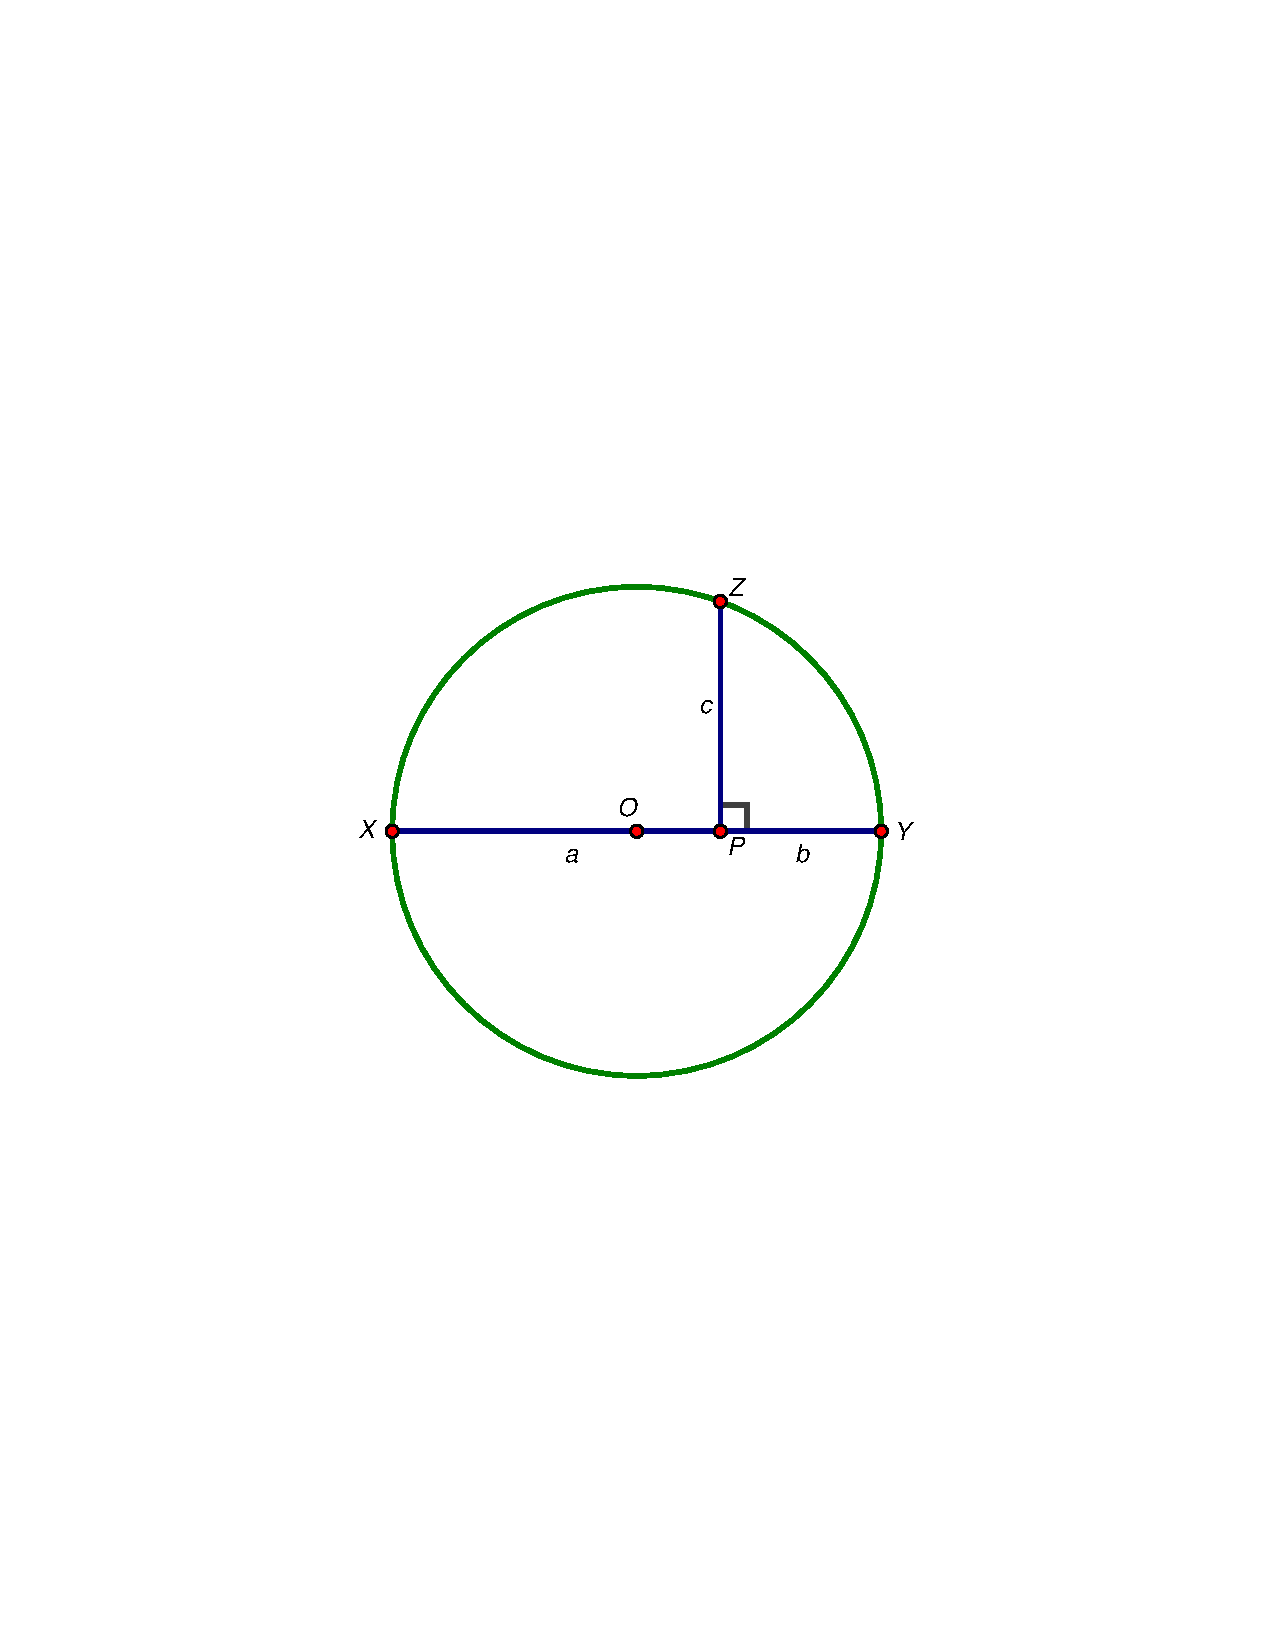
\includegraphics[scale=0.7]{Means}$$
\begin{enumerate}
\item Show that $c=\sqrt{ab}$.  
\item Then use the figure to explain the Arithmetic-Geometric Mean Inequality: 
$$\frac{a+b}{2} \ge \sqrt{ab}$$
\item Why is this called the Arithmetic-Geometric Mean Inequality?  
\end{enumerate}
\end{prob}





\newpage

\section{Supplemental Problems}

\subsection{Parametric Equations}


\begin{prob} 
Consider a nonzero vector defined by the ordered pair $(a,b)$. If $\|
(a,b)\|$ is the magnitude of this vector, \textbf{use algebra} to
explain why
\[
\frac{(a,b)}{\|(a,b)\|}
\]
is a new vector whose magnitude is $1$ and whose direction is the same
as $(a,b)$.
\end{prob} 

\begin{prob}
Suppose you have a parametric plot defined by $x(t)$ and $y(t)$.
\begin{enumerate}
\item Compare and contrast the plots of
\[
\bigg(x(t),y(t)\bigg)\qquad\text{and}\qquad\bigg(x(t-6),y(t-6)\bigg).
\]
\item Suppose that there are two bugs whose positions are given by:
\[
\mathrm{bug}_1(t) = \bigg(x(t),y(t)\bigg)\qquad\text{and}\qquad\mathrm{bug}_2=\bigg(x(t-6),y(t-6)\bigg).
\]
where $t$ represents time in seconds. Describe what happens as $t$
runs from $0$ seconds to $36$ seconds.

\item Now suppose that there are two bugs whose positions are given
  by:
\[
\mathrm{bug}_1(t) = \bigg(x(t),y(t)\bigg)\qquad\text{and}\qquad\mathrm{bug}_2=\bigg(x(t)-6,y(t)-6\bigg).
\]
where $t$ represents time in seconds. Describe what happens as $t$
runs from $0$ seconds to $36$ seconds.
\end{enumerate}
\end{prob} 

\begin{prob}
Find the intersection of the lines
\begin{align*}
x_1(t) &= -6 + 9t & x_2(t) &= 3+t \\
y_1(t) &= 3-2t &  y_2(t) &= -4-2t 
\end{align*}
If $(x_1(t),y_1(t))$ gives the position of $\mathrm{jogger}_1$ and
$(x_2(t),y_2(t))$ gives the position of $\mathrm{jogger}_2$, what is
the significance of the point of intersection of these lines, from the
perspective of the joggers?
\end{prob}

\begin{prob}
A bug moves according to the following parametric equations, where t is measured in seconds and $x$ and $y$ are measured in centimeters:  $x = 2t^2$, $y = t-2$.  (Suppose $t$ can be any real number.)   
\begin{enumerate}
\item Describe the path of the bug.  
\item Is the bug's position a function of time?  
\item On the path, is $y$ a function of $x$?  
\item Is $x$ a function of $y$?  
\item If you know one of $x$, $y$, or $t$, can you determine the other two?  How does this question relate to the previous two questions?  
\item In school mathematics, students are often given a graph and asked, ``Is it a function.''  Explain why this is a poor question.  What better questions could you ask?  
\end{enumerate}
\end{prob}

\subsection{Absolute Value, Distance, and City Geometry}
\begin{prob}
Consider the following equations:  
\setlength{\arraycolsep}{12pt}
\setlength{\extrarowheight}{3pt}
\[
\begin{array}{cccc}
x^2-y^2=0    &   x^2=y^2   &   |y|=|x|   &   y= \pm x \\
(x-y)(x+y)=0  &   x= \pm y   &   y = \pm|x|   & x = \pm|y|
\end{array}
\]
\begin{enumerate}
\item Which equations are equivalent to which other equations?  Say how you know.  (Be sure to state what it means for the equations to be equivalent.)
\item For each set of equivalent equations, graph the solution set, and describe how each of the equations provides a different way about thinking about that solution set.  
\end{enumerate}
\end{prob}

\begin{prob}
Distance formulas and circle equations across dimensions.  
\begin{enumerate}
\item What is the (Euclidean) distance formula in 2 dimensions, on the $xy$-plane?  
\item What is the distance formula in 3 dimensions?
\item What is the distance formula in 1 dimension?
\item Write an equation of the circle of radius $r$ and center $(a, b)$.  
\item Explain how a circle is a one-dimensional figure living in a two-dimensional ``space.''
\item In three-dimensional space, write an equation of the two-dimensional ``circle'' of radius $r$ and center $(a, b, c)$.  
\item In one-dimensional space, write an equation of the zero-dimensional ``circle'' of radius $r$ and center $a$.  
\end{enumerate}
\end{prob}

%\begin{prob}
%Distances across dimensions.  
%\begin{enumerate}
%\item Find all numbers that are equidistant from 3 and 8.  
%\item Find all points $(x, y)$ that are equidistant from $(3, 0)$ and $(8, 0)$.  
%\item Find all points $(x, y, z)$ that are equidistant from $(3, 0, 0)$ and $(8, 0, 0)$.  
%\item Find all real numbers that are twice as far from 3 as they are from 8.
%\item Find all points $(x, y)$ that are twice as far from $(3, 0)$ as they are from $(8, 0)$.
%\item Find all points $(x, y, z)$ that are twice as far from $(3, 0, 0)$ as from $(8, 0, 0)$.
%\end{enumerate}
%\end{prob}
%
%4.5.  One way of solving problems 4a and 4d is as follows: 
%(1)	Use a distance formula from problem 3 to express the distances from x to 3 and from x to 8; 
%(2)	Use an equation to relate the distances from part (1); and 
%(3)	Thinking of the two sides of the equation as functions, graph the two functions and look for intersections of the graphs. 
%How can you use this approach to predict how many solutions you will find?

\begin{prob} 
Recall the method in Euclidean geometry of constructing an equilateral triangle on a given segment.  Suppose a ``city geometry compass'' draws a city geometry circle.  Imagine using such a ``city geometry compass'' below.  
\begin{enumerate}
\item Construct a ``city geometry equilateral triangle'' on the segment defined by the
  points $(0,0)$ and $(4,0)$. Explain your steps.
\item Now construct a ``city geometry equilateral triangle'' on the segment defined by the
  points $(0,0)$ and $(2,2)$. Explain your steps.
\item Will the construction always give a (unique!) equilateral triangle? What does ``unique'' mean in this context? Give a detailed discussion.  
\end{enumerate}
\end{prob} 

%
%\begin{prob} 
%Consider a nonzero vector defined by the ordered pair $(a,b)$. If $\|
%(a,b)\|$ is the magnitude of this vector, \textbf{use algebra} to
%explain why
%\[
%\frac{(a,b)}{\|(a,b)\|}
%\]
%is a new vector whose magnitude is $1$ and whose direction is the same
%as $(a,b)$.
%\end{prob} 

\subsection{Measurement}
\begin{prob}
If the perimeter of a rectangle is 20 feet, what is the most one can say about the rectangle's area?  If the perimeter of any simple closed 2-dimensional shape is 20 feet, what is the most anyone can say about its area?
\end{prob}

\begin{prob}
If the surface area of a rectangular prism is 20 square feet, what is the most one can say about the prism's volume?  If the surface area of any simple closed 3-dimensional shape is 20 square feet, what is the most one can say about its volume? 
\end{prob}

\begin{prob}
Why do cute furry animals curl up to stay warm in the winter?  Why are most ugly desert reptiles long and skinny?
\end{prob}

\begin{prob}Simple closed curve A is contained entirely inside simple closed curve B.  
\begin{enumerate}
\item True or False:  The area enclosed by A is less than the area enclosed by B. Explain
\item True or False:  The perimeter of A is less than the perimeter of B. Explain.  
\end{enumerate}
\end{prob}

\begin{prob}
Is it correct to say that``area is length times width''?  Think about what these three quantities mean.  When would it be correct in the numerical sense and why?  (Make sure you use the meaning of multiplication.)   
\end{prob}

\begin{prob}
The apothem of a regular polygon is defined to be the shortest distance from the center of the polygon to an edge.
\begin{enumerate}
\item There is a nice relationship between the apothem, perimeter, and area for a regular polygon.  See if you can find it. (Hint:  Split the polygon into congruent triangles from its center and find the area of the polygon in terms of the apothem and perimeter.)  You can assume you know the area of a triangle $=\frac{1}{2}$(Length of Base)(Length of Height).
\item What does this result say about the area of a circle?  Explain. (Assume you know the circumference of a circle is $2\pi(radius)$.)
\end{enumerate}
\end{prob}

\begin{prob}
 Is it correct to say that ``volume is length times width times height''? What must be true about a figure so that the numerical volume can be more easily measured by ``area times height''?
\end{prob}

\begin{prob}
Are there figures for which there is no formula for measuring length, area, and volume?  Explain.  What does your answer to this question imply about the teaching of geometric measurement?
\end{prob}

\begin{prob}
Convert 25 yards to meters (and 25 meters to yards) using ``2.54 cm in each inch'' as the only Metric-English unit conversion.  Explain the conversion using the meanings of multiplication and division (In particular, when you divide, what kind of division is it?)
\end{prob}

\begin{prob}
Now convert 25 square yards to square meters and 25 square meters to square yards.  Do the same with cubic yards and cubic meters.
\end{prob}

\fixnote{Add problems about oriented area, planimeter.}  

\begin{prob}
TIMSS 1995 problem about changing a border for equal areas. 
\end{prob}

\begin{prob}
Using oriented area, given a quadrilateral $ABCD$, and any point $O$ in the plane, $$\text{area} ABCD = \text{area}\triangle OAB + \text{area}\triangle OBC + \text{area}\triangle OCD + \text{area}\triangle ODA.$$
\end{prob}
  
\begin{prob}
A parallelogram with vertices at $(0,0)$, $(a,b)$, $(c,d)$, and $(a+c,b+d)$ has (oriented) area $ad-bc$. 
% Draw a big rectangle around it, and subtract the stuff we don't want.
% Row reduction of a matrix as parallelograms with same base, same height.  Area (and determinant) is constant.  
\end{prob}

\begin{prob}
If $ad-bc = 0$, then $(a,b)$ and $(c,d)$ are parallel.  What about the converse?  
\end{prob}




\end{document}
